\section{Metoder}
En kort præsentation af de to mest dominerende arbejdsmetoder der er anvendt.\\

I dette projekt er der anvendt metoder indlært gennem et tidligere projekt. Værktøjerne er de værktøjer som gruppen føler sig trygge ved og som gruppen føler bidrager mest til processen. 
\subsection{SCRUM}
I gruppens implementering af SCRUM startes der med at lave en produktbacklog, som er den kunden ser.  Derefter planlægges det første sprint. Et sprint spænder over 2 uger. Når et sprint starter bliver opgaver overført fra backloggen til sprintet. Når nye opgaver bliver sat på sprintet bliver opgaven vurderet for hvor stort et omfang den har. Derefter diskuteres der hvilke opgaver de forskellige dele af gruppen skal lave. En gang om ugen laver man et SCRUM-Meeting. Her bliver fulgt op på opgaver lavet i løbet af ugen samt tilføjelse af nye opgaver. Nye sprint startes hver anden uge og alle de opgaver der ikke er færdige, når sprintet er slut, overføres til næste sprint.\\
I projektet er der i alt 7 sprint. På \textit{Figur ~\ref{fig:SCRUM}} vises det 2. sprint.
\begin{figure}[H]
\centering
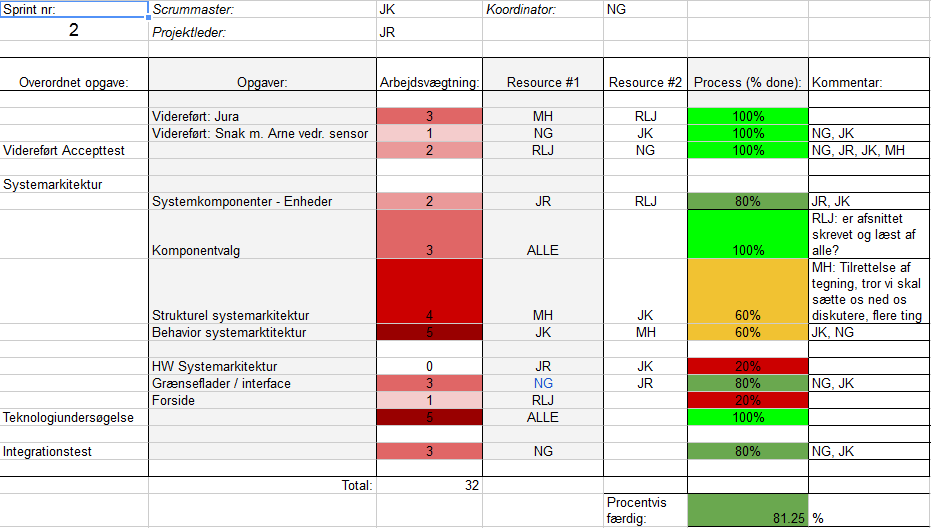
\includegraphics[width=0.9\textwidth]{billeder/SCRUM1}
\caption{Sprint 2}
\label{fig:SCRUM}
\end{figure}
Sprintet er afsluttet og man kan se hvordan nogle opgaver er færdige og hvordan resten skal overføres til næste sprint. Billedet illustrerer også hvordan planlægningen er opbygget. Forklaring af statusfarver er vist på \textit{Figur~\ref{fig:SCRUM2}}
\begin{figure}[H]
\centering
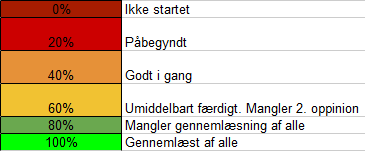
\includegraphics[width=0.5\textwidth]{billeder/SCRUM2}
\caption{Forklaring af sprint points}
\label{fig:SCRUM2}
\end{figure}
\subsection{V-model}
\begin{figure}[H]
\centering
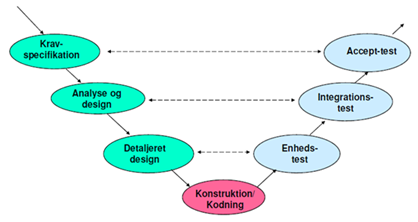
\includegraphics[width=0.5\textwidth]{billeder/vmodel}
\caption{V modellen}
\label{fig:vmodel}
\end{figure}
Vi har valgt at anvende V modellen som udviklingsmodel. Dette muliggør iterative processer hvilket er optimalt for vores udviklingstil.